\chapter{PENGAJUAN PROPOSAL PROYEK II}
\section{Tujuan}
Untuk	memudahkan	pelaksanaan	pekerjaan	Proyek II,	mahasiswa	diwajibkan	mengajukan	proposal	 Proyek II dalam	 bentuk	 daring dan	 opsional	 luring(kesepakatan	 dengan	 calon	pembimbing).	 Proposal	 ini	 akan	 menjadi	 acuan	 bagi	 mahasiswa,	 dosen	 pembimbing	maupun	Koordinator	Proyek	II	dalam	pelaksanaan	pekerjaan	Proyek II.

\section{Isi Proposal Luring}
Proposal	Proyek II luring	berisi	:

\begin{enumerate}
  \item \textbf{Judul	proyek}	dalam	bentuk	cover (\textit{format	ada	di	lampiran	1}).
  
  \item \textbf{Lembar	persetujuan	proposal} (\textit{format	ada	di	lampiran	2}).
	
  \item \textbf{Abstrak}  
  
  \item \textbf{Daftar Isi} termasuk

  \begin{enumerate}
    \item Daftar Gambar
    \item Daftar Tabel
    \item Daftar Simbol
    \item Daftar Singkatan Kata
  \end{enumerate}
  
  \item \textbf{BAB I Pendahuluan}
  
  \begin{enumerate}
  	\item \textbf{Latar Belakang} (berisi	 latar	 belakang	 dari	 pengerjaan	 proyek,	 dibuat	 narasi	minimal	3	paragraf).
  	
  	\item \textbf{Identifkasi Masalah} (berisikan	hal	– hal	yang	menjadi	masalah	untuk	dibuat	proyek	tersebut).
  	
  	\item \textbf{Tujuan} (berisikan	 tujuan	 pembuatan	 proyek,	 berisi	 latar	 belakang	 dari pengerjaan proyek,	dibuat	narasi	minimal	3	paragraf).
  	
  	\item \textbf{Ruang Lingkup} atau	 Batasan	 Masalah (berisikan batasan-batasan	 pekerjaan	agar	dapat	selesaisesuai	dengan	jadwal	pekerjaan).
  	
  	\item \textbf{Jadwal Kegiatan Pekerjaan Proyek}, dibuat \textit{timeline} per minggu.
  \end{enumerate}
  
  \item \textbf{BAB II Landasan Teori} \\
   \textbf{(} berisikan uraian \textbf{tentang	 teori	 yang	mendukung} Objek	PROYEK	 2.	\textbf{Harus	 jelas	 sumber	 rujukannya	 dari mana}.  Sumber	 yang	 baik	 adalah	jurnal	 ilmiah,	 artikel	 ilmiah,	 buku,	 dll.	 	Disarankan	 untuk \textbf{tidak	 mengambil	 sumber	seperti	WebBlog,	Wikipedia,	dll.).}	

	\item \textbf{DAFTAR PUSTAKA}
\end{enumerate}

\section{Proposal Daring}
Peserta	 Proyek	 2	 sudah	menyiapkan	github,	 video	log	 dan	 blog	 untuk	 dikirimkan	melalui	formulir	 yang	 disediakan.	 Harap	 diperhatikan	 setiap	 detil	 tata	 cara	 pembuatan	 github,	 video	log	dan	blog	yang	standar	di	BAB	selanjutnya.

\subsection{Github}
Peserta	 dalam	 satu	 kelompok	 yang	 terdiri	 dari	 2	 orang	membuat	 akun	 github	 masingmasing.	 Kemudian	 buatlah organisasi	 baru	 dengan	 nama	 kelompok	 yang	 ada	 kaitannya	
dengan	topik	proposal	yang	diajukan.


\begin{figure}[H]
    \centering
    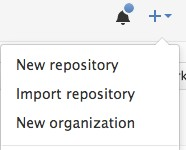
\includegraphics[scale=0.7]{figures/git.jpg}
    \label{git}
\end{figure}

Lengkapi	 data	 dan	 email	 kemudian	 Create	 Organization,	 kemudian	 masukkan	 username	anggota	untuk	kolaborasi dan	user	kordinator	proyek	2	awangga	sebagai	admin.	Setelah	itu	buat repository	 masing-masing	 anggota	 di	 dalam	 organisasi	 baru	 tersebut	 sesuai	 dengan	judul	proposal	masing-masing	sebagai	contoh	bisa	anda	buka	di \url{https://github.com/d4TI}

\begin{figure}[H]
    \centering
    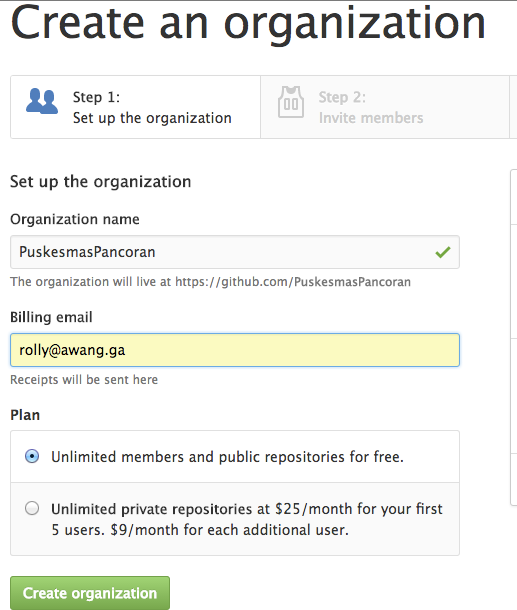
\includegraphics[scale=0.7]{figures/11.png}
    \label{11}
\end{figure}

Didalam	repositori	yang	didalamnya	terdapat	: \par 
\textbf{File	README.md} \par 
Berisi	 perkenalan	 diri	 nama,NPM,	 kelas,	 jurusan,	 kampus	 dan	 Judul	 dan	 deskripsi	 dari	Proyek	2	yang	diajukan	dalam	bahasa	Inggris	ditulis	dengan	script	markdown. \par 

\textbf{File	Licence} \par 
File	ini	dipilih	ketika	pertama	kali	repositori	dibuat. \par 

\textbf{Folder	doc} \par
Didalam	 folder	 doc	 ada	 folder	 proposal	 yang	 berisi	 tiga	 file	 isi	 dari	 proposal	 yaitu	abstraksi.md,	 BAB-I.md,BAB-II.md	 yang	 diisi	 dengan	 proposal	 peserta	 dalam	 bentuk	
markdown \par 

\textbf{Folder	img} \par 
Ini	adalah	folder	untuk	menaruh	gambar-gambar	yang	dimasukka	kedalam	proposal \par 

Pada	menu	Issues	peserta harus	mengisi	Milestone	dengan	jadwal-jadwal	penting	yang	ada	di	buku	petunjuk	ini.

\begin{figure}[H]
    \centering
    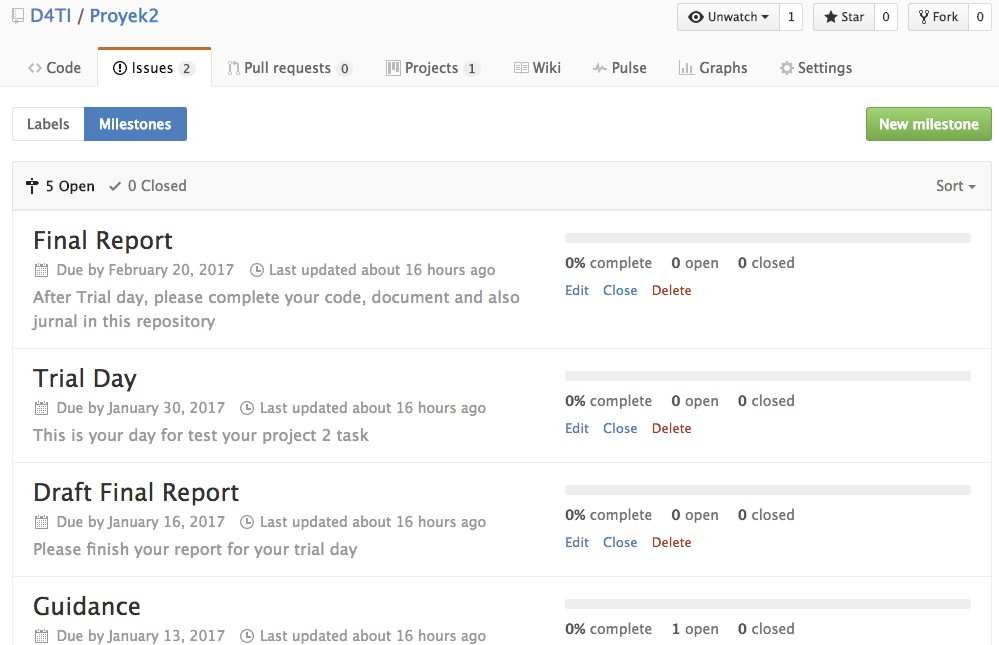
\includegraphics[scale=0.5]{figures/22.jpg}
    \label{22}
\end{figure}

Pada	menu	Project	peserta	membuat	New	Project	dengan	nama	Project	2	yang	didalamnya	berisi	Kanban	atau	scrum	dengan	kolom,	To	Do,	Doing,	Testing,	Done


\begin{figure}[H]
    \centering
    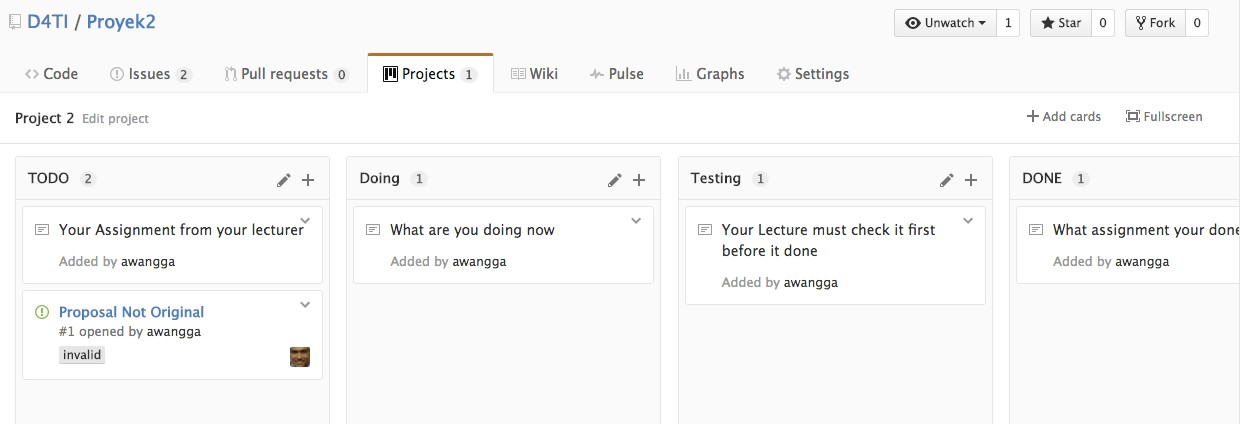
\includegraphics[scale=0.5]{figures/33.jpg}
    \label{33}
\end{figure}

Semua	 hasil	evaluasi	dan	 bimbingan(peserta	membantu	input	 sendiri	 hasil	 bimbingan) di	lempar	 ke	 menu	 issues dengan	 setting	 label	 sesuai	 dengan	 kriteria	 masalah,	 milestone	
sesuai	dengan	target	jadwal	yang	dikejar	assignment	untuk	ditujukan	kepada	peserta	yang	mana.	 Setelah	issues	masuk,	 kemudian	 oleh	 peserta	 dimasukkan	 ke	 kartu	 Scrum	 Todo	 di	menu	Project \textrightarrow Project	2dengan	klik	+Add	Cards. Ambil	kartu	yang	sedang	anda	kerjakan	pindahkan	ke	Doing,	setelah	selesai	masuk	ke	testing	begitu	seterusnya	hingga	kolom	To	Do	habis	 kartunya.	 Jika	pembimbing	menyetujui	pekerjaan	maka	 kartu	peserta	pindahkan	 ke	Done	dan	commit	file	yang	bersangkutan	dengan	menggunakan	hashtag	nomor	isu	agar	isu	
ter	 close	 secara	 otomatis(bukan	 di	 close	 dari	 tombol	 close	 di	 github).	 Semua	 perubahan	dan	 penambahan	 file	 di	 dalam	 repository \textbf{harus	 menggunakan	 aplikasi	 git	 bash} yang	standar	 sesuai	 dengan	 penjelasan	 di	 BAB	 selanjutnya,\textbf{dilarang	 keras	 melakukan	penambahan	 dan	 perubahan	 di	 web	 github	 secara	 langsung} dibuktikan	 dengan	perekaman	 pembuatan	 untuk	 disertakan	 di	 video	 log. Semua	 isi	 proposal	 di	 3	 file markdown \textbf{wajib	di	scan	plagiarism} 	hasil	screensot	plagiarisme	di	 taruh di	dalam	 folder	img/proposal dan	disertakan	link	tersebut	di	blog. Sebagai	contoh	repository	bisa	dilihat	di	
\url{https://github.com/D4TI/Proyek2/}.

\subsection{Video}
Peserta	juga	membuat	video	standar	sesuai	dengan	arahan	di	BAB selanjutnya.

\subsection{Blog}
Buat	 blog standar	 sesuai	 dengan	 arahan	 di	 BAB	 selanjutnya. Yang	 didalamnya	 sudah	diembed	video	dan	link	repository	serta	link	hasil	scan	plagiarism.
\\
\\
Proposal	di	submit	melalui	url	:
\\ \url{http://s.id/Proyek2}
\section{Reviewer}

\textit{Reviewer} adalah \textit{ team} yang	 terdiri	 dari	 2 orang	 yang	 mempunyai	 kepakaran	 di	 bidang	masalah	yang	akan	di	\textit{review}. \textit{\textbf{Team reviewer}} akan	ditunjuk	oleh	Koordinator	Proyek,	hasil evaluasi	yang	dilakukan	oleh \textit{\textbf{Reviewer}} adalah	mutlak,	dengan	ketentuan	sebagai	berikut	:

\begin{enumerate}
\item Dua Reviewer	menolak	maka	Proposal	Proyek	ditolak.
\item Satu Reviewer	menolak,	satu	menerima	maka	Proposal	Proyek	ditolak.
\item Dua Reviewer	menerima	maka	Proposal	Proyek	diterima.
\end{enumerate}

\section{Pengesahan	Proposal Proyek	II}
Persetujuan	 atas	 proposal	 oleh	 Koordinator	 Proyek	 II	 didasarkan	 pada	 hasil	\textit{Review} oleh \textit{Review},	yang	dibuktikan	dengan	diterbitkannya	surat	persetujuan	pelaksanaan	Proyek	II	kepada	 mahasiswa	 yang	 bersangkutan	 dan	 tembusan	kepada	 dosen	 pembimbing.	 Tanpa	surat	 persetujuan	 tersebut,	 pelaksanaan	 Proyek	 II	 bukan	 menjadi	 tanggung	 jawab Koordinator	Proyek II dan	tidak	akan	diproses	kelanjutannya.